\section{Minecraft}

Minecraft é um jogo eletrônico do tipo sandbox que permite a interação com um ambiente aberto através da manipulação de blocos. Para além do aspecto recreativo, o jogo possui um sistema de simulação física e lógica denominado \textbf{Redstone}. Este sistema permite a criação de circuitos complexos, funcionando como uma abstração prática de sistemas digitais reais. Devido a essa característica, o Minecraft é amplamente utilizado como ferramenta educacional para demonstrar conceitos de eletrônica digital, lógica booleana e arquitetura de computadores. Para este projeto, foi utilizado o minecraft Java Edition 1.18.2.

\imgbig{Minecraft.jpg}{Capa do Minecraft}

\subsection{A Unidade de Tempo: Game Ticks e Redstone Ticks}
Diferente de circuitos eletrônicos físicos, onde a propagação é quase instantânea, o processamento da Redstone é discreto e baseado em \textit{ticks}. É fundamental distinguir as duas unidades de medida utilizadas no motor do jogo:

\begin{itemize} 
	\item \textbf{Game Tick (GT):} É a unidade mínima de processamento do jogo. O Minecraft busca processar 20 GT por segundo, o que significa que 1 GT equivale a \textbf{0,05 segundos} (50ms).
	 \item \textbf{Redstone Tick (RT):} A maioria dos componentes lógicos opera em intervalos de 2 Game Ticks. Portanto, 1 RT equivale a 0,1 segundos. Este é o "passo" padrão para a atualização de estados em circuitos síncronos dentro do jogo. 
\end{itemize}
\subsection{Componentes Vanilla}

Embora seja uma abstração simplificada, o funcionamento do sistema de redstone apresenta paralelos com circuitos digitais reais, especialmente no que diz respeito à propagação de sinais e controle lógico. 

Esse sistema interno é bem complexo e cheio de detalhes, o que segue é um resumo dos principais conceitos e componentes da redstone, que serão necessários para compreensão do projeto. Para mais detalhes, é recomendável consultar a wiki do jogo \cite{minecraft_wiki_redstone} \cite{minecraft_wiki}.

\subsubsection{Pó de Redstone}

A poeita de redstone atua como meio de transmissão de sinal, análogo a fios em circuitos eletrônicos. Ela transporta um valor de intensidade que varia de 0 a 15, sendo interpretado, em muitos casos, como sinal lógico binário (0 ou 1) ou como hexadecimal (0-15).

A propagação ao longo da poeira é instantânea (0 RT), porém o sinal perde 1 unidade de força a cada bloco percorrido, limitando a transmissão a no máximo 15 blocos sem o uso de repetidores. 

\begin{figure}[H]
   	\centering
   	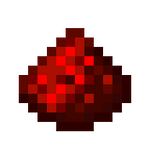
\includegraphics[width=0.2\linewidth]{images/redstone.png}
  	 \caption{Redstone}
   	\label{fig:redstone}
\end{figure}

\subsubsection{Tocha de Redstone}

A tocha de Redstone, além de energizar blocos adjacentes quando está ligada, funciona como um inversor lógico. Quando o bloco em que está apoiada recebe energia, ela desliga; quando não recebe, permanece ligada. Esse comportamento permite a inversão de sinais dentro de circuitos.

\begin{figure}[H]
   	\centering
   	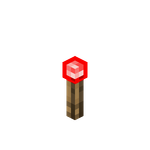
\includegraphics[width=0.3\linewidth]{images/redstone-torch.png}
  	 \caption{Tocha de Redstone}
   	\label{fig:tocha-de-redstone}
\end{figure}

\subsubsection{Repetidor de Redstone}

O repetidor é um componente multifuncional projetado para transmitir, amplificar e atrasar sinais. Ele possui duas funções avançadas essenciais para o projeto: 

	 \textbf{Ajuste de Delay:} Pode ser configurado manualmente para introduzir um atraso de 1, 2, 3 ou 4 RTs. 

\begin{figure}[H]
   	\centering
   	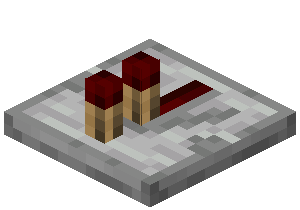
\includegraphics[width=0.3\linewidth]{images/Redstone_Repeater.png}
  	 \caption{Repetidor de Redstone}
   	\label{fig:redstone-repeater}
\end{figure}

	 \textbf{Trava:} Se um repetidor for energizado lateralmente por outro repetidor ou comparador, ele "trava" seu estado atual, ignorando mudanças na entrada traseira. Essa propriedade é frequentemente utilizada para criar memórias de forma compacta.

\begin{figure}[H]
   	\centering
   	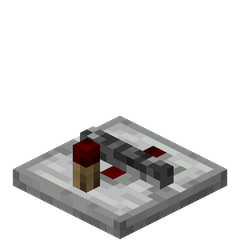
\includegraphics[width=0.34\linewidth]{images/Locked_Redstone_Repeater.png}
  	 \caption{Repetidor de Redstone Travado}
   	\label{fig:locked-redstone-repeater}
\end{figure}

\subsubsection{Comparador de Redstone}

O comparador é o componente mais sofisticado do sistema \textit{vanilla}, permitindo operações aritméticas e de comparação com um atraso constante de 1 RT. Ele opera em dois modos:

 \textbf{Modo Comparação (Tocha frontal apagada):} A saída só é ativada se o sinal traseiro for maior ou igual ao maior sinal lateral. 

\textbf{Modo Subtração (Tocha frontal acesa):} A saída emite uma intensidade igual à diferença entre o sinal traseiro e o maior sinal lateral ($saida = max(0, back - max(side inputs))$). Se o resultado for negativo, a saída é 0.

\begin{figure}[H]
   	\centering
   	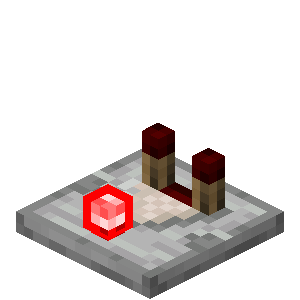
\includegraphics[width=0.34\linewidth]{images/redstone-comparator.png}
  	 \caption{Comparador de Redstone}
   	\label{fig:redstone-comparator}
\end{figure}

\subsubsection{Input/Output}

Componentes como botões, alavancas e placas de pressão atuam como entradas (inputs), fornecendo sinais ao sistema. Já lâmpadas de Redstone e pistões podem ser utilizados como saídas (outputs), respondendo ao estado lógico do circuito.

\subsection{Mods}

Embora o sistema de redstone presente na versão vanilla do jogo já permita a construção de circuitos digitais relativamente complexos, algumas limitações práticas, como atraso de propagação, dificuldade de depuração e alta complexidade estrutural, motivam o uso de modificações (mods) que expandem essas capacidades.

Esses mods introduzem ferramentas e abstrações que aproximam o ambiente do jogo de um contexto mais controlado e analisável, semelhante ao de sistemas digitais reais ou simuladores de hardware. Foi utilizado o Fabric 0.19.1-1.18.2

\subsubsection{Carpet}

O mod Carpet fornece ferramentas avançadas de análise e instrumentação do jogo. Entre suas funcionalidades, destacam-se a medição de desempenho, inspeção de ticks e controle fino do comportamento do sistema.

Essas capacidades permitem observar com maior precisão a execução de circuitos de redstone, facilitando a identificação de gargalos, condições de corrida e inconsistências temporais.

\subsubsection{Wired Redstone}

O mod Wired Redstone introduz um sistema de fiação estruturado que substitui a redstone tradicional por conexões mais organizadas e previsíveis.

Diferentemente da redstone vanilla, esses fios não sofrem degradação de sinal ao longo da distância, eliminando a necessidade de repetidores.

\textbf{Principais itens:}
\begin{itemize}
    \item \textbf{Red Alloy Wire}: fio condutor básico sem perda de sinal.
    \item \textbf{Insulated Wire}: fios isolados por cor, permitindo múltiplos sinais independentes em paralelo.
    \item \textbf{Bundled Cable}: permite transmitir vários sinais simultaneamente em um único bloco (barramento multi-bit).
    \item \textbf{Gate Components}: componentes lógicos (AND, OR, NOT, etc.) integrados ao sistema de fios.
	\item \textbf{Repetidor de Redstone}: o mod adiciona uma alternativa do repetidor de redstone \textit{vanilla} com personalização do atraso em ticks gerado.
\end{itemize}

\begin{figure}[H]
   	\centering
   	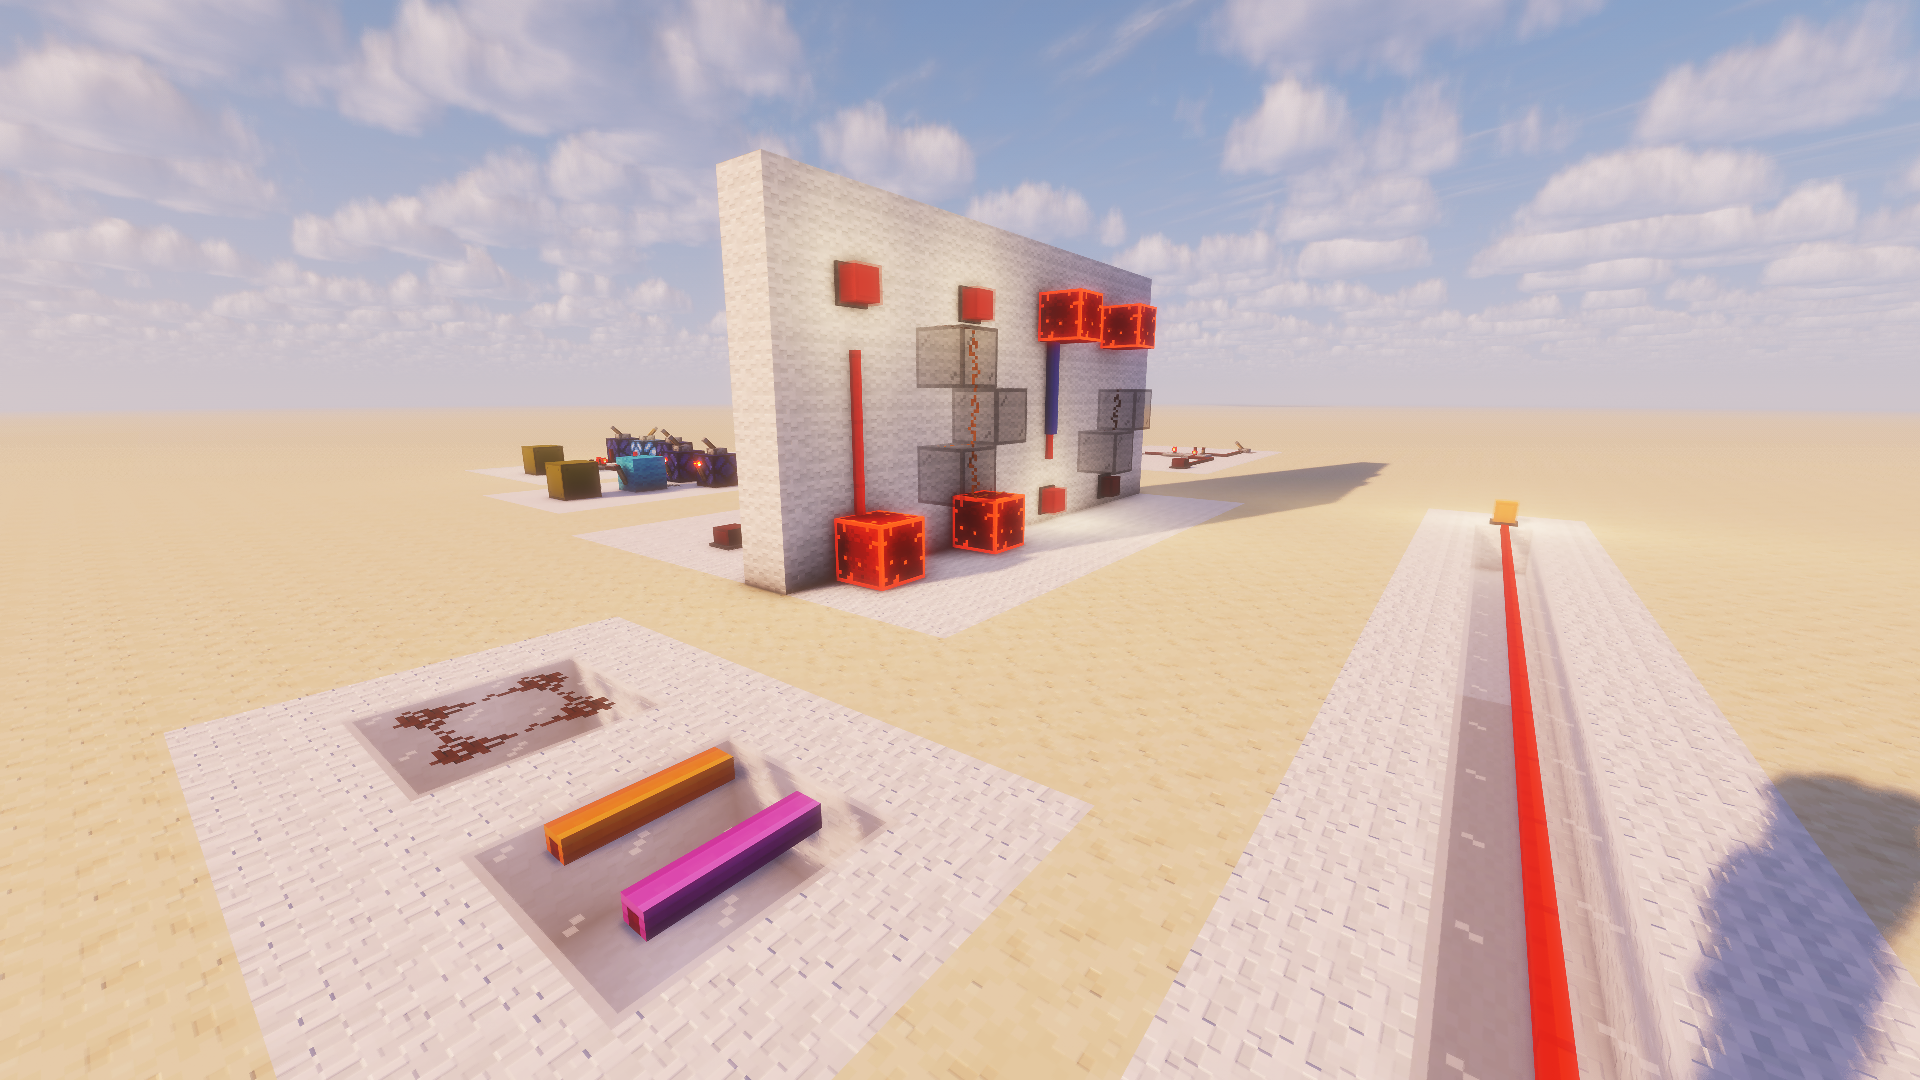
\includegraphics[width=0.7\linewidth]{images/wired-redstone.png}
  	 \caption{Fios de Redstone}
   	\label{fig:wired-redstone}
	%{\footnotesize Fonte: \url{https://autoctrls.com/datasheet-transistor/}}
\end{figure}


\subsubsection{Wireless Redstone}

O mod Wireless Redstone introduz comunicação sem fio entre componentes, eliminando completamente a necessidade de conexões físicas.

O funcionamento segue o modelo de transceptores: um transmissor envia um sinal em uma determinada frequência/canal, e receptores configurados na mesma frequência reproduzem esse sinal.

\textbf{Principais itens:}
\begin{itemize}
    \item \textbf{Transmitter}: envia sinais de redstone para um canal específico.
    \item \textbf{Receiver}: recebe sinais de um canal e os converte em saída de redstone.
    \item \textbf{Frequency Selector}: define o canal de comunicação entre dispositivos.
\end{itemize}

\begin{figure}[H]
   	\centering
   	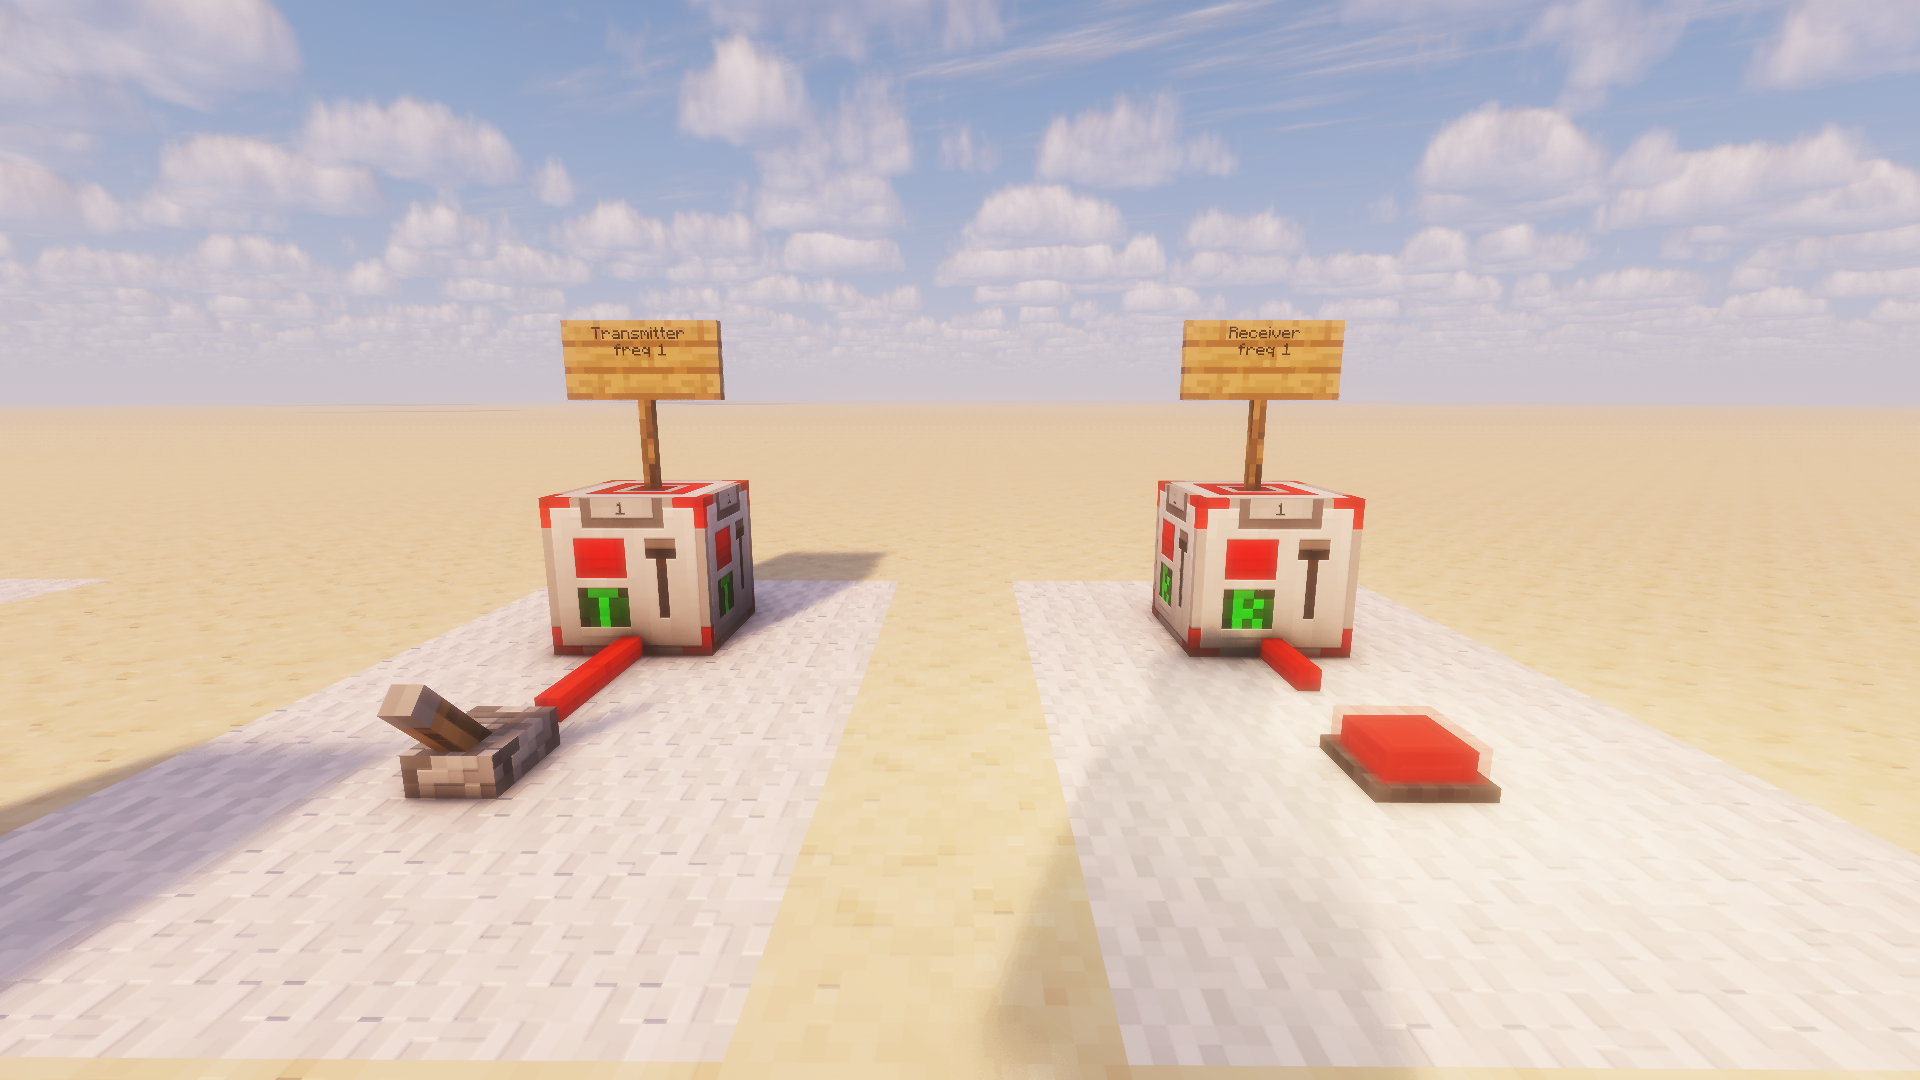
\includegraphics[width=0.7\linewidth]{images/wireless-redstone.png}
  	 \caption{Transmissor e Receptor}
   	\label{fig:wireless-redstone}
	%{\footnotesize Fonte: \url{https://autoctrls.com/datasheet-transistor/}}
\end{figure}
\subsection{Portas Lógicas de Redstone}

No Minecraft, a implementação de portas lógicas não depende diretamente de transistores físicos, mas sim de abstrações comportamentais do sistema de redstone.

\subsubsection{Or}

No jogo, a porta Or é a mais simples de todas, se nossas variáveis $A$ e $B$ propagam em fios opostos, para fazer uma porta Or, basta juntar estes dois fios na saida $X$, já que qualquer um deles pode energizar $X$.

\begin{figure}[H]
   	\centering
   	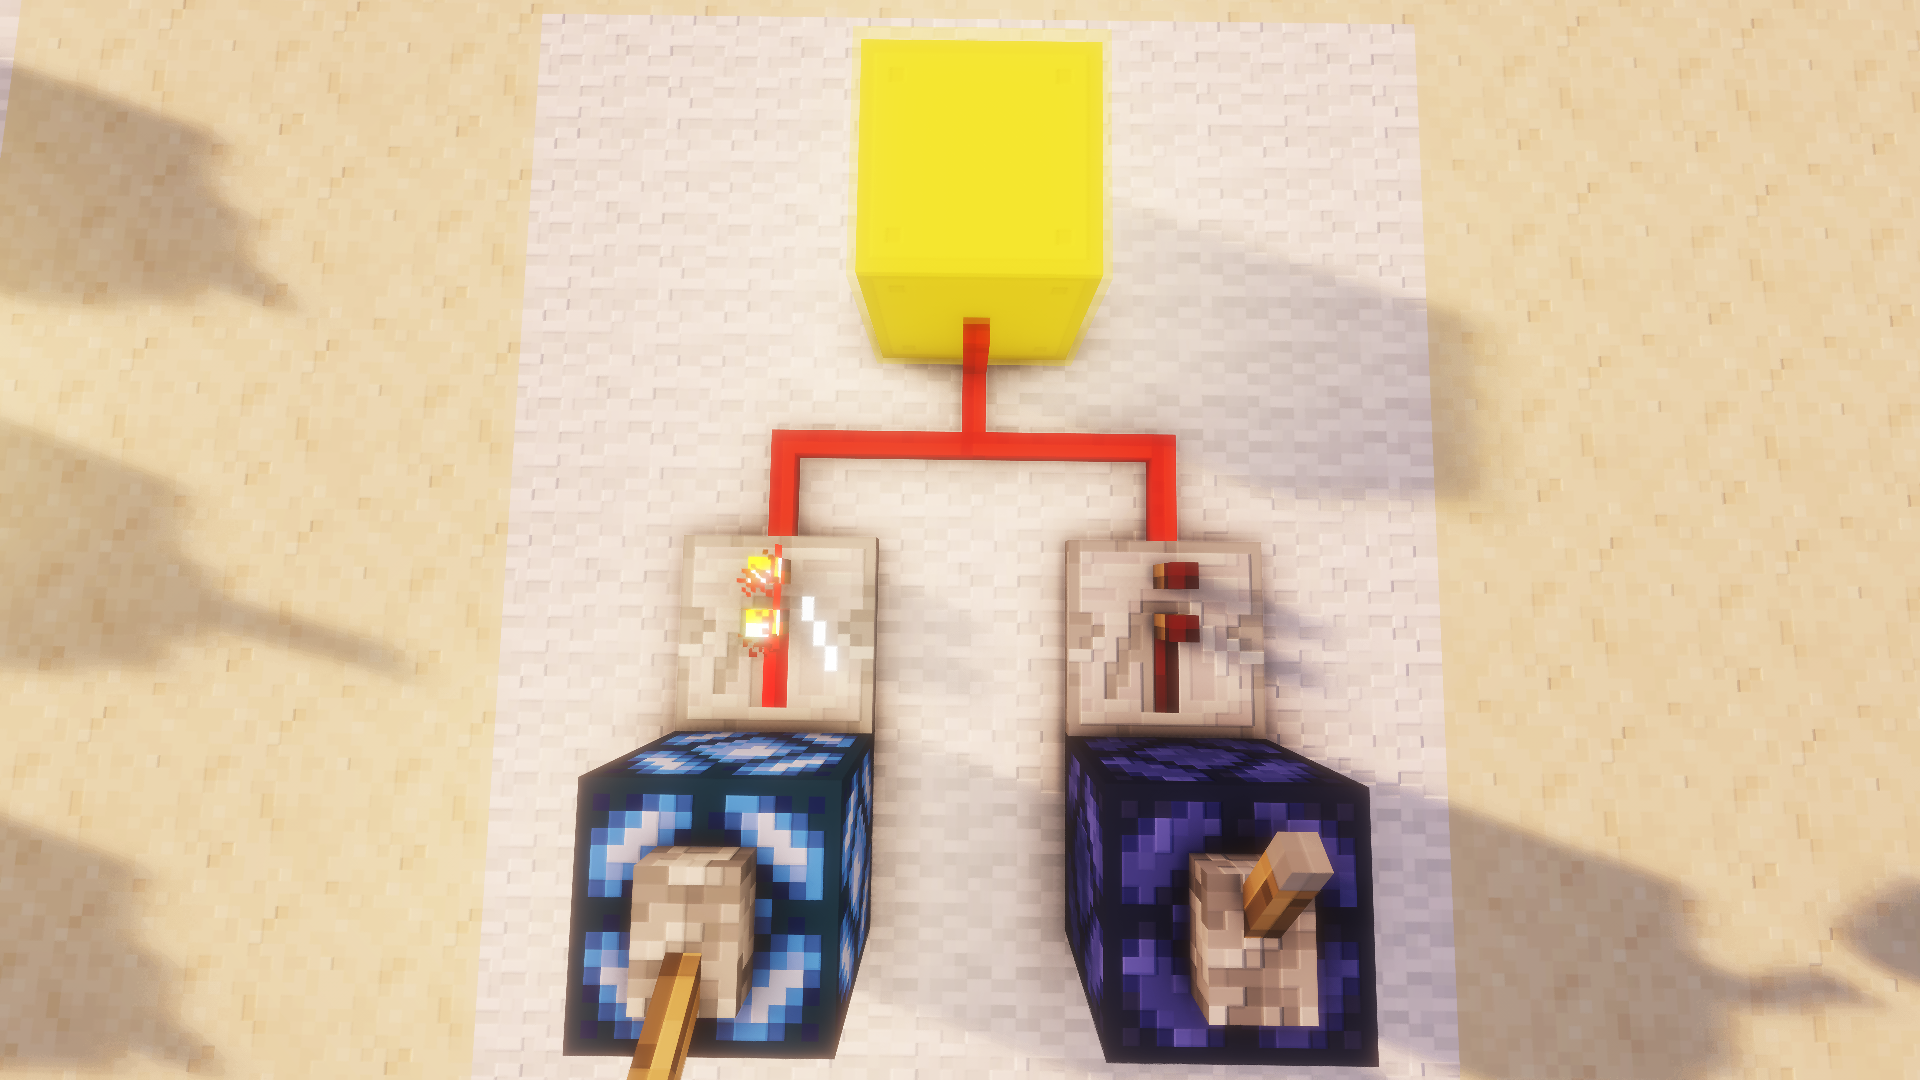
\includegraphics[width=0.7\linewidth]{images/or-redstone.png}
  	 \caption{Porta Or de Redstone}
   	\label{fig:or-redstone}
	%{\footnotesize Fonte: \url{https://autoctrls.com/datasheet-transistor/}}
\end{figure}

\subsubsection{Not}

A porta lógica NOT (ou inversor) é uma das implementações mais fundamentais em circuitos de Redstone. No Minecraft vanilla, ela é tradicionalmente construída utilizando uma tocha de redstone.

O funcionamento baseia-se no fato de que a tocha de redstone inverte o estado do sinal de entrada:
quando não há energia na entrada, a tocha permanece ligada, emitindo sinal na saída; quando a entrada é energizada, a tocha desliga, interrompendo o sinal.

\begin{figure}[H]
    \centering
    \includegraphics[width=0.7\linewidth]{images/not-redstone.png}
    \caption{Porta Not de Redstone utilizando tocha}
    \label{fig:not-redstone}
\end{figure}

Em algumas modificações do jogo (como o mod citado “Wired Redstone”), a porta NOT pode ser implementada como um componente dedicado, aumentando a eficiência espacial em circuitos complexos.

\begin{figure}[H]
    \centering
    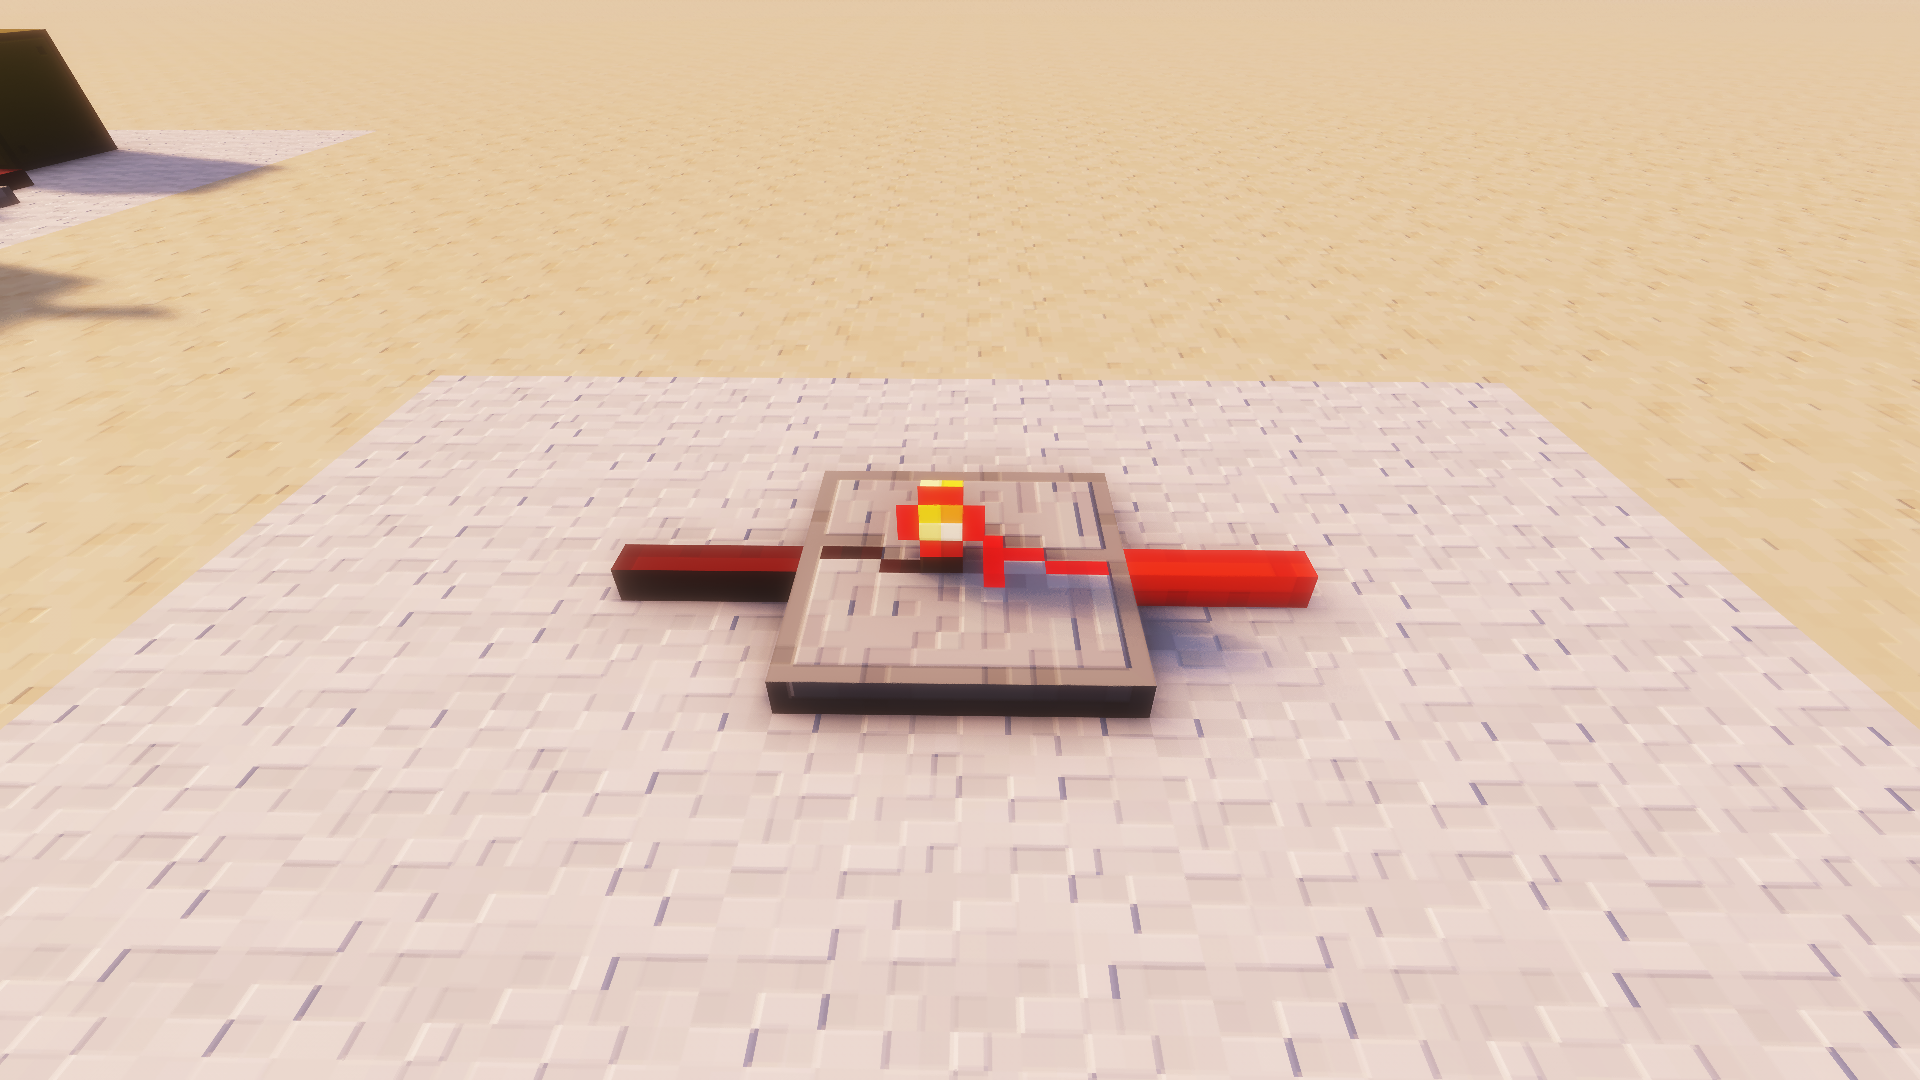
\includegraphics[width=0.7\linewidth]{images/not-wired-redstone.png}
    \caption{Porta Not de Redstone do mod Wired Redstone}
    \label{fig:not-wired-redstone}
\end{figure}

\subsubsection{And}

No jogo \textit{vanilla}, assim como na vida real, existem várias formas de se implementar o portão and. Entretanto, a forma mais utilizada no jogo é derivada da lei de De Morgan: 

\begin{center}
$(\lnot(p \land q) \equiv (\lnot p \lor \lnot q)) \iff ((p \land q) \equiv \lnot (\lnot p \lor \lnot q)) $
\end{center}

\begin{figure}[H]
    \centering
    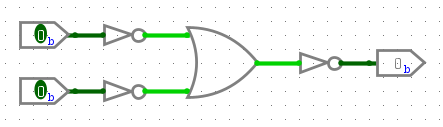
\includegraphics[width=0.7\linewidth]{images/and-circuit-alternative.png}
    \caption{Circuito alternativo para a porta And}
    \label{fig:and-circuit-alternative}
\end{figure}

\begin{figure}[H]
    \centering
    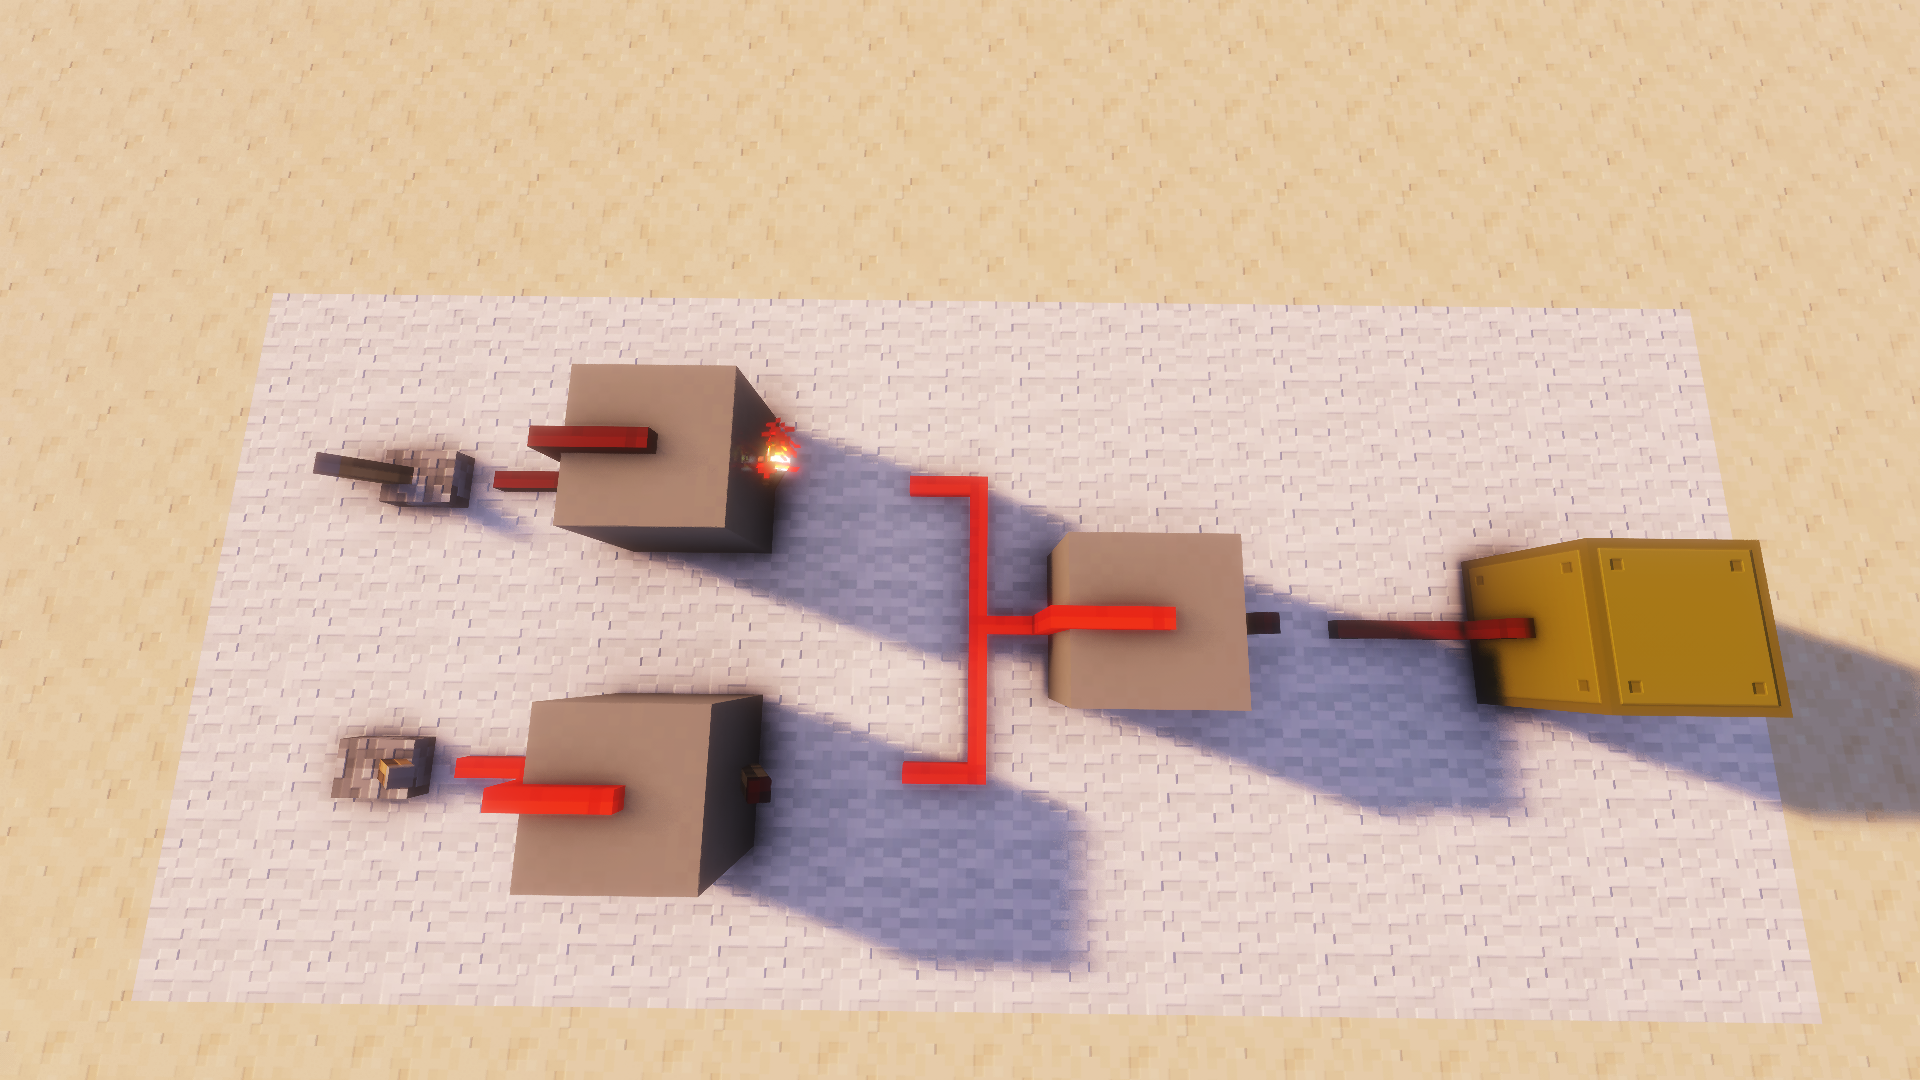
\includegraphics[width=0.7\linewidth]{images/and-redstone.png}
    \caption{Circuito And de Redstone para Minecraft Vanilla}
    \label{fig:and-redstone}
\end{figure}

\begin{figure}[H]
    \centering
    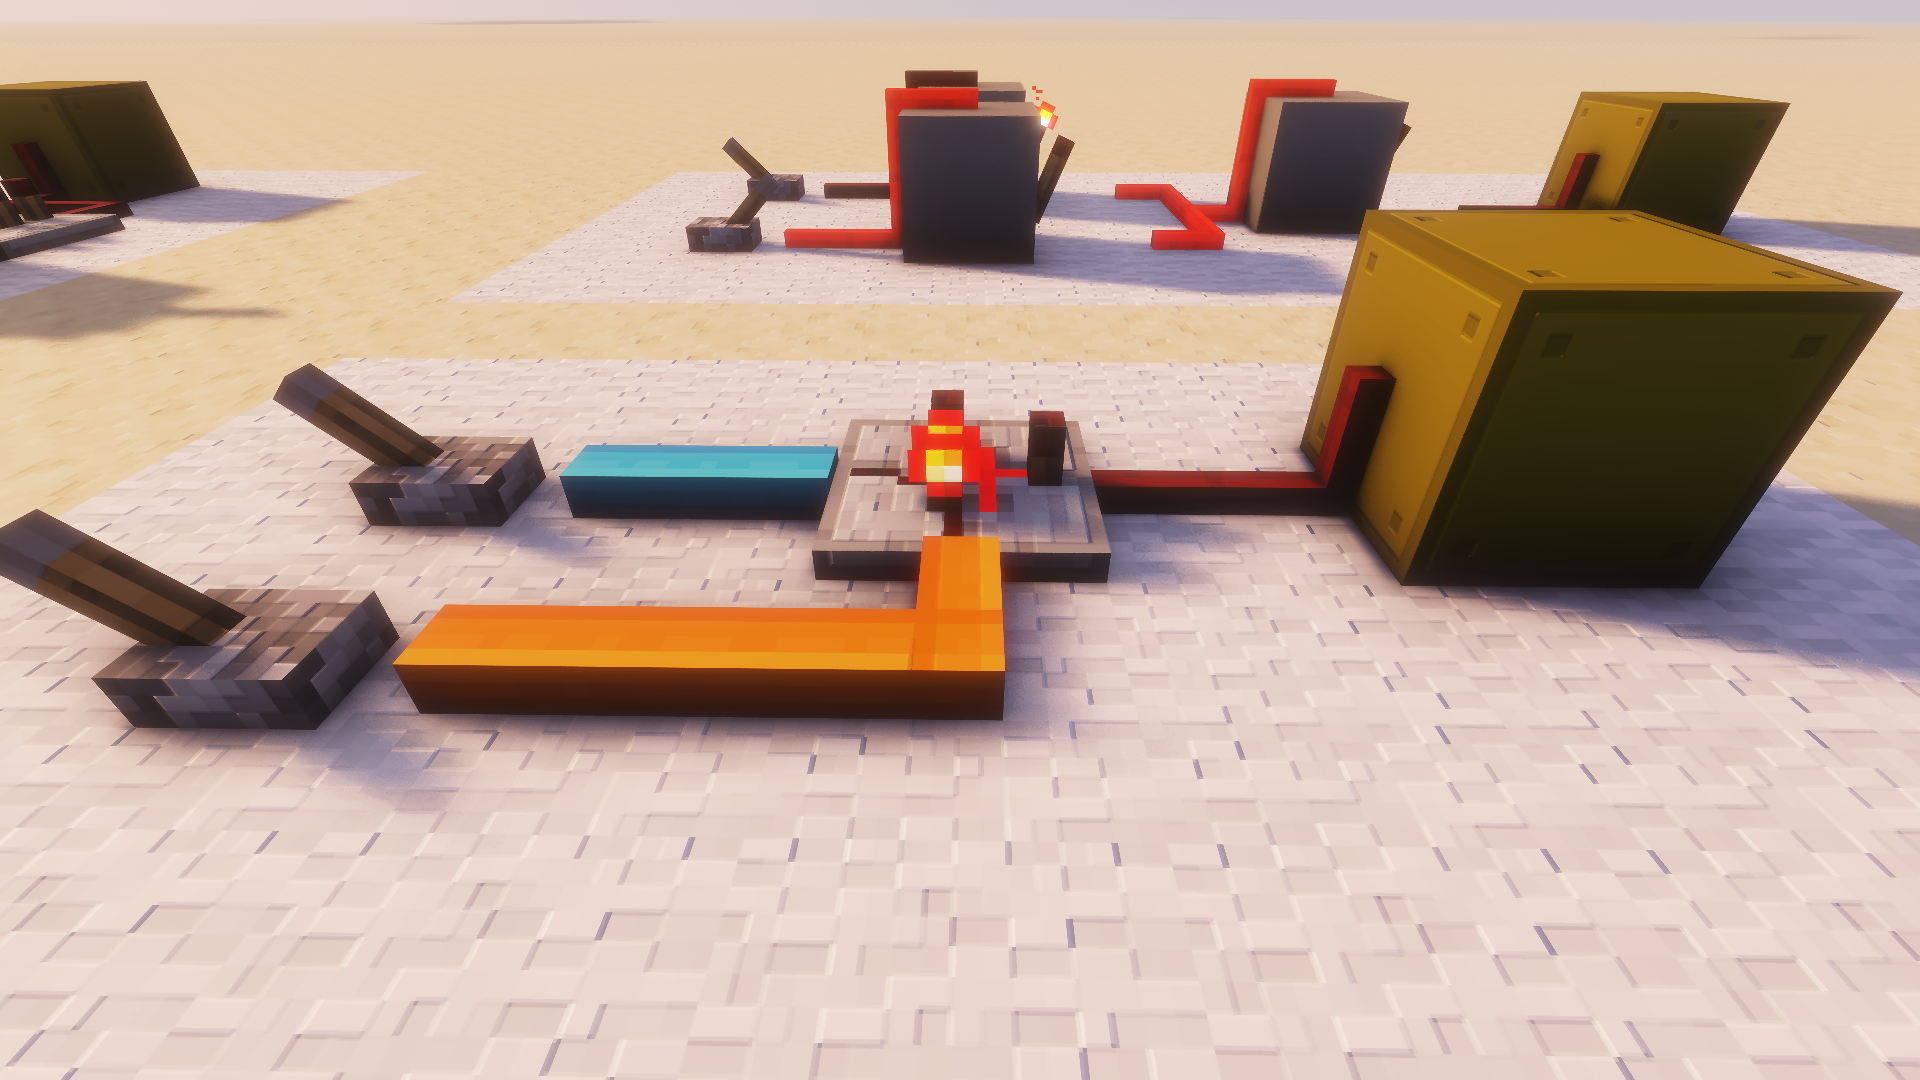
\includegraphics[width=0.7\linewidth]{images/and-wired-redstone.png}
    \caption{Circuito Integrado And Wired Redstone}
    \label{fig:and-wired-redstone}
\end{figure}

\subsubsection{Xor}



